% CREATED BY DAVID FRISK, 2018
\chapter{BehaviorStudio}

Una vez definidas todas las herramientas que se van a utilizar para el desarrollo de este proyecto, se dedicará este capítulo para cubrir de forma extensa y precisa una de las patas fundamentales del mismo: la plataforma de \textit{machine learning} BehaviorStudio \footnote{https://jderobot.github.io/BehaviorStudio/}.
Para ello, se dará primero una visión general de la arquitectura de la aplicación, para acto seguido describir todos los detalles de la implementación llevada a cabo, así como los problemas que han surgido y las soluciones aportadas.

Este capítulo está dividido en 4 secciones principales que abordarán una pequeña introducción de la aplicación, el diseño de la arquitectura, los principales componentes que la componen y el modo de ejecución distribuido.

\section{Introducción}

BehaviorStudio es una plataforma de \textit{machine learning} de comportamientos basados en redes neuronales que permite conectar distintos \textit{software} inteligentes a un robot tanto real como simulado. La plataforma está ideada principalmente para la conducción autónoma a través del control visual utilizando como sensores principales las cámaras a bordo del robot, pero está preparada para el soporte de diferentes robots como: drones, robots industriales, domésticos, etc, y para diferentes sensores y actuadores. Esta plataforma está ideada para proporcionar una infraestructura accesible y flexible que permita ejecutar diferentes comportamientos complejos en coches autónomos implementados con diferentes técnicas como: \textit{deep learning} (redes de clasificación, regresión, recurrentes, LSTMs, ...), \textit{reinforcement learning} e incluso programación manual utilizando librerías de visión como OpenCV.

Esta plataforma está íntegramente desarrollada en Python dado que es uno de los lenguajes más utilizado por la comunidad en el desarrollo de aplicaciones de aprendizaje automático, al disponer de gran cantidad de librerías y herramientas creadas por la comunidad científica, tales como Numpy, Pytorch, OpenCV, etc.

Esta plataforma surge de la inspiración de otra plataforma similar en características denominada \textit{DetectionStudio} \footnote{https://jderobot.github.io/DetectionStudio/} desarrollada por miembros de la asociación JdeRobot \footnote{https://jderobot.github.io}.

\noindent BehaviorStudio proporciona la siguiente funcionalidad:

\begin{itemize}
    \item \textbf{Carga de cerebros}. Se pueden seleccionar diferentes modelos de comportamiento (modelos pre-entrenados) para su evaluación en la misma ejecución del programa.
    \item \textbf{Modificación 'en caliente'}. BehaviorStudio permite la modificación del código del cerebro en ejecución sin necesidad de parar el programa, realizando carga dinámica de los algoritmos que gobiernan el robot.
    \item \textbf{Ejecución en diferentes plataformas}. La plataforma soporta entornos de ejecución locales (simulación en Gazebo) y remotos (robots reales).
    \item \textbf{Visualización}. Se incorpora la visualización de diferentes sensores como la cámara RGB o el láser.
    \item \textbf{Modo de ejecución distribuida}. Se permite ejecutar la lógica y la visualización en diferentes computadores (modo \textit{headless}), para permitir así que la capa de lógica corra empotrada en los robots, mientras que la capa de visualización se ejecute en un computador externo.
    \item \textbf{Creación de \textit{datasets}}. Se pueden grabar conjuntos de datos utilizando \textit{ROSBags} asociados a \textit{topics} de ROS.
\end{itemize}

La implementación de esta plataforma es flexible, lo que permite incorporar nueva funcionalidad como visualización de otros tipos de sensores de forma sencilla, o de nuevos marcos de trabajo como Tensorflow.

\section{Arquitectura \textit{software}}

El diseño de BehaviorStudio se puede ver en la Figura \ref{fig:architecture}. Como se puede observar, al tratarse de una aplicación que incorpora visualización, se ha implementado una arquitectura Modelo-Vista-Controlador (MVC). Se ha elegido esta arquitectura porque distingue muy bien la parte de lógica y la parte de visualización, disminuyendo el acoplamiento de componentes y facilitando la cohesión de los mismos. La parte inferior de esa infografía, bajo la etiqueta "\textit{Robotic Platform}", ilustra la capacidad que tiene BehaviorStudio de conectar con robots reales o simulados indistintamente, cambiando únicamente la configuración de la aplicación. Esto se consigue gracias a la estandarización en las comunicaciones que ofrece ROS en forma de \textit{topics}, para: tanto recibir la información sensorial de los sensores del robot, como para comandar órdenes a sus actuadores.

Los principales componentes de esta aplicación son los que se aprecian en la Figura \ref{fig:architecture}. Por simplicidad, este diagrama sólo muestra los componentes principales de BehaviorStudio, obviando el módulo de grabación de datasets que se explican en la sección \ref{sec:redata}. Se puede apreciar que los componentes de los sensores/actuadores, el piloto y el cerebro forman parte del Modelo en el MVC, y a su vez se observa el módulo controlador perteneciente a la capa controladora, y por último la interfaz de usuario (UI) que pertenece a la capa de vista del MVC. En la siguiente sección se explican detalladamente cada uno de los componentes \textit{software} implementados en esta aplicación.

\begin{figure}
  \centering
  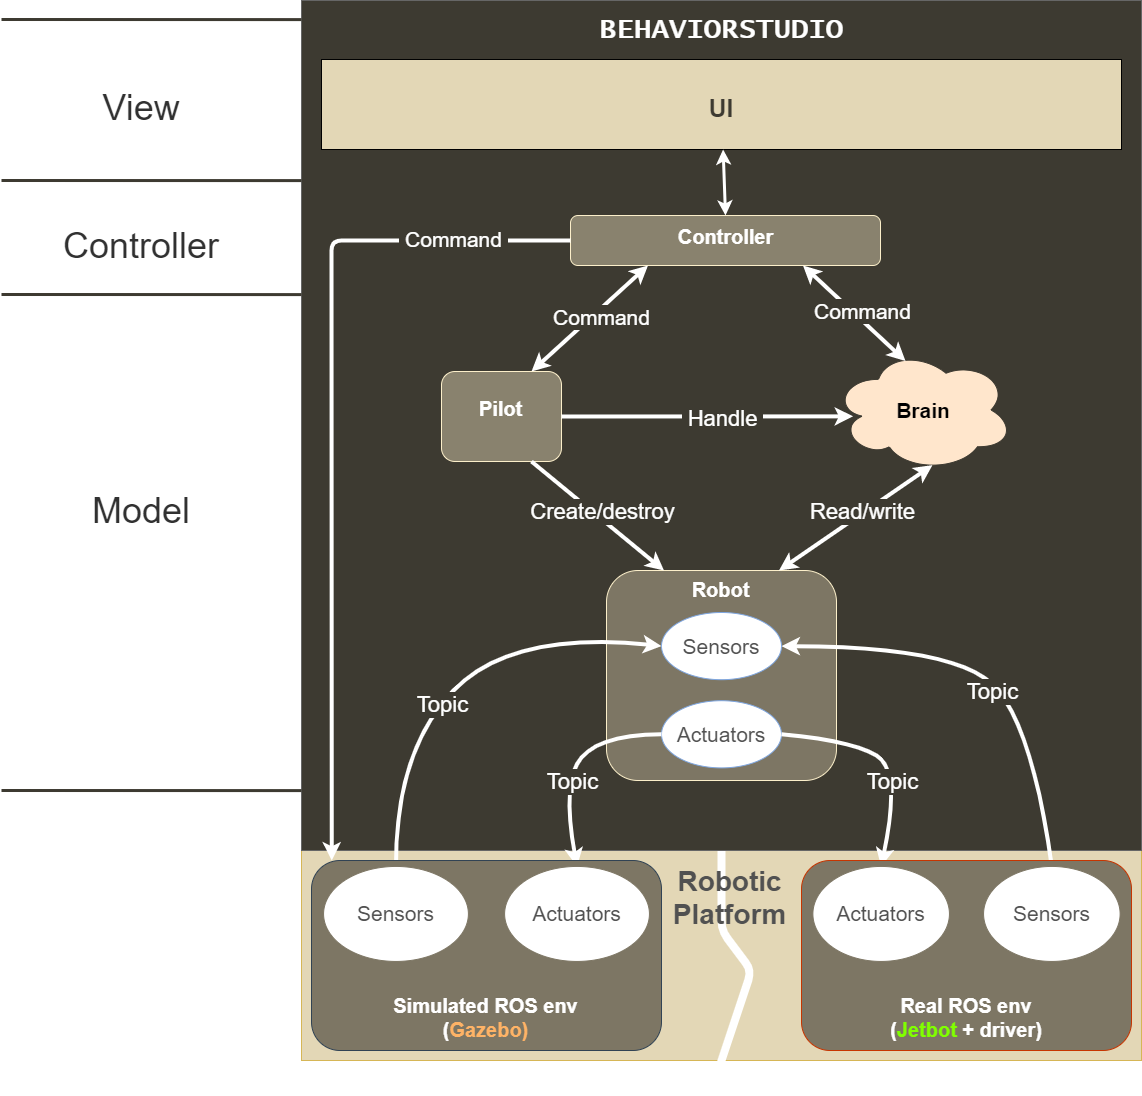
\includegraphics[width=.7\linewidth]{img/arquitectura}
  \caption{Arquitectura de BehaviorStudio}
  \label{fig:architecture}
\end{figure}

\section{Componentes}
\label{sec:components}

En esta sección se detallan los diferentes componentes que componen la arquitectura de la aplicación, tal como ilustra la figura \ref{fig:architecture}. Cada componente se explicará en una sección diferente para mayor claridad, para posteriormente abordar el modo de ejecución distribuida.

\subsection{Driver}
\label{sec:driver}

\textcolor{blue}{No sé si incluir esta sección. Es como el programa principal, que gestiona la ejecución, pero no sé si es interesante para el propósito de la memoria. Si es así la completo.}

El punto de entrada de la misma es el \textit{driver}. Este módulo gestiona la ejecución de toda la aplicación. Entre sus tareas se encuentra:

\begin{itemize}
    \item \textbf{Inicialización de componentes}. El \textit{driver} se encarga de crear todos los componentes necesarios para la ejecución del programa, entre ellos: el piloto,el interfaz de usuario, el simulador y el controlador.
    \item \textbf{Destrucción de componentes}. También se encarga de destruir todos los elementos creados cuando termina la ejecución.
\end{itemize}

\subsection{Piloto}
\label{sec:pilot}

El módulo principal de la aplicación es el piloto. Esta pieza se encarga principalmente de la creación tanto del robot (sensores y actuadores) como del cerebro que va a comandar al robot. El piloto tiene un hilo de ejecución que se actualiza periódicamente cada $ 60 ms $, donde en cada iteración se ejecuta una llamada al cerebro que esté cargado en ese momento, para que este tome una decisión en función del escenario en el que se encuentre en cada instante. En otras palabras, cada $ 60\ ms $ se realiza una llamada al método \lstinline{execute()} del cerebro cargado, que capturará información del sensor o sensores, realizará una inferencia sobre la información capturada y tomará una decisión sobre cómo debe actuar el robot en ese momento. Esto permite que el control sea reactivo, ya que se toman decisiones en cada instante en función de las percepciones del robot. Esto da pie a múltiples implementaciones de control visual tanto de lazo abierto (sin realimentación sobre el sistema) como de lazo cerrado (con realimentación sobre el sistema), todas reactivas.

Otra característica que se apuntó en la introducción es que BehaviorStudio permite el cambio de cerebros, además de cambios en el código fuente de forma dinámica sin necesidad de reiniciar la aplicación, esto es, en tiempo de ejecución. Es el piloto se encarga de realizar la carga y descarga de estos cerebros de forma dinámica que el usuario indique a través del interfaz de usuario.

En la Figura \ref{fig:pilotuml} se ilustra un diagrama de clases reducido de la clase piloto. Esta clase dispone de los métodos necesarios para crear un robot y cargar cerebros a placer de forma dinámica, además del hilo de ejecución principal.

\begin{figure}
  \centering
  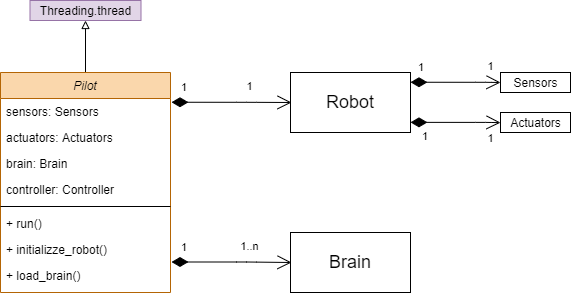
\includegraphics[width=.6\linewidth]{img/pilotuml}
  \caption{Diagrama de clases UML del componente pioto}
  \label{fig:pilotuml}
\end{figure}

\subsection{Robot - Sensores y actuadores}

Un elemento fundamental de los robots en general son sus sensores y actuadores, ya que sin ellos el robot sería incapaz de percibir (o sensar) ni de interactuar con el entorno. Por lo tanto, uno de los pilares principales de BehaviorStudio es la implementación del soporte de los sensores y actuadores del robot.

La implementación de este componente es sencilla, ya que se trata de un paquete de Python que incluye sendas clases \textit{Sensors} y \textit{Actuators}, que recibe una lista de sensores y actuadores con sus respectivos \textit{topics} desde el fichero de configuración de la aplicación. En la Figura \ref{fig:robouml} se puede ver un pequeño diagrama de clases UML que ilustra parcialmente la implementación de este componente. Esta implementación es flexible, ya que permite incluir una cantidad arbitraria de sensores y/o actuadores sin tener que modificar el código, solamente modificando el fichero de configuración.

La forma en la que se construye un objeto sensor o actuador es especificando qué tipo de sensor se quiere construir, un identificador y el \textit{topic} de ROS asociado al publicador o subscriptor de ese sensor/actuador. Adicionalmente se podrá especificar configuración extra para cada sensor/actuador (requerirá la modificación del código). Todo esto se especifica a través de un fichero de configuración en formato YAML. En el Fragmento \ref{yml_rob} se puede ver un ejemplo de configuración para el robot F1.

\begin{tabular}{c}
\begin{lstlisting}[caption={Ejemplo de configuración en formato YAML},label=yml_rob]
Robot:
    Sensors:
        Cameras:
            Camera_0:
                Name: 'camera_0'
                Topic: '/F1ROS/cameraL/image_raw'
        Pose3D:
            Pose3D_0:
                Name: 'pose3d_0'
                Topic: '/F1ROS/odom'
    Actuators:
        Motors:
            Motors_0:
                Name: 'motors_0'
                Topic: '/F1ROS/cmd_vel'
                MaxV: 3
                MaxW: 0.3
    BrainPath: 'brains/f1/brain_f1_opencv.py'
    Type: 'f1'
\end{lstlisting}
\end{tabular}

Se pueden agregar tantos sensores o actuadores como tenga el robot en uso, pudiendo identificar cada uno de ellos con el identificador proporcionado en la etiqueta \textit{Name}. Los tipos de sensores soportados en la versión actual de BehaviorStudio son: cámaras RGB, láser, y pose3D. Por su parte, los actuadores soportados son: motores.

\begin{figure}
  \centering
  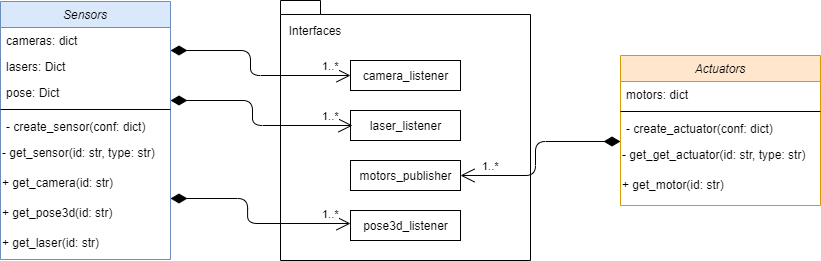
\includegraphics[width=1\linewidth]{img/robotuml}
  \caption{Diagrama de clases UML del componente Robot}
  \label{fig:robouml}
\end{figure}

\subsection{Cerebros neuronales}
\label{sec:brainnets}

El módulo de cerebros neuronales (llamado \textit{Brains}), es la pieza fundamental de BehaviorStudio, ya que es aquí donde residen los algoritmos que gobernarán a los robots. Como se aprecia en la Figura \ref{fig:architecture}, éste módulo conecta con los sensores y actuadores de los robots y es gestionado por el piloto, como se explicó en la sección \ref{sec:pilot}. Además tiene comunicación con el controlador, para que el usuario pueda interactuar con la carga de modelos, pausar o reanudar su ejecución, o modificar el código fuente todo en tiempo de ejecución. La conexión con los sensores y actuadores del robot, es fundamental para que el cerebro que esté en ejecución pueda realizar las inferencias a partir de los datos sensoriales, y comandar acciones al robot en función de las predicciones realizadas por las redes neuronales que gobiernan los robots.

\begin{figure}
\centering
\begin{forest}
  for tree={
    font=\ttfamily,
    grow'=0,
    child anchor=west,
    parent anchor=south,
    anchor=west,
    calign=first,
    inner xsep=7pt,
    edge path={
      \noexpand\path [draw, \forestoption{edge}]
      (!u.south west) +(7.5pt,0) |- (.child anchor) pic {folder} \forestoption{edge label};
    },
    % style for your file node 
    file/.style={edge path={\noexpand\path [draw, \forestoption{edge}]
      (!u.south west) +(7.5pt,0) |- (.child anchor) \forestoption{edge label};},
      inner xsep=2pt,font=\small\ttfamily
                 },
    before typesetting nodes={
      if n=1
        {insert before={[,phantom]}}
        {}
    },
    fit=band,
    before computing xy={l=15pt},
  }  
[brains
  [brain\_handler.py,file]
  [f1
    [brain\_f1\_dummy.py,file]
    [brain\_f1\_classification.py,file]
    [...,file]
  ]
  [car
    [brain\_car\_dummy.py,file]
    [...,file]
  ]
  [drone
    [...,file]
  ]
  [...,file]
]
\end{forest}
\caption{Estructura de directorios de cerebros neuronales}
\label{fig:braindir}
\end{figure}

Todos los módulos cerebro comparten un interfaz común, que "obliga" a seguir un estándar que democratiza todas las implementaciones que realicen los usuarios; así, un ejemplo de implementación de un cerebro sería como el que se muestra en el Fragmento \ref{brainex}. Como se puede observar, este cerebro es muy sencillo, el comportamiento que genera en el robot es que éste gira sobre su propio eje a $ 0.8\ rad/s $. 

Cada cerebro debe implementar una clase llamada \textit{Brain} instanciando en el constructor los sensores y actuadores del robot identificados por su nombre (en el caso del Fragmento \ref{brainex} \lstinline{camera_0} y \lstinline{motors_0} para la cámara y los motores respectivamente), además de una instancia del manejador de cerebros llamada \lstinline{handler}, que gestiona las comunicaciones con el módulo controlador. Dispone de un método \lstinline {update_frame()} que se encarga de actualizar la información que llega al interfaz de usuario con la visualización de los datos del sensor pertinente cada vez que se invoca. Por último, la función \lstinline {execute()}, es la encargada del bucle principal de ejecución que es llamada desde el módulo Piloto a un ritmo de ejecución determinado (ver sección \ref{sec:pilot}). 

En el caso de la Figura \ref{brainex}, cada vez que el método \lstinline{execute()} es invocado, se ejecutará lo siguiente: que el robot no avance (línea 13), que el robot gire sobre sí mismo a una velocidad de $0.8\ rad/s$ (línea 14), obtener una imagen de la cámara a bordo del robot (línea 15) y actualizar la información que se mostrará en la interfaz de usuario con la imagen capturada (línea 16). En la última instrucción, el primer argumento es \lstinline{frame_0}, que es el nombre del cuadro donde se mostrará la imagen capturada de la cámara del robot en el interfaz de usuario. Esto se explicará con más detalle en la sección \ref{sec:ui}.

\begin{tabular}{c}
\begin{lstlisting}[caption={Ejemplo de implementación de cerebro no neuronal},label=brainex,style=Python] 
class Brain:
    
    def __init__(self, sensors, actuators, handler=None):
       
        self.camera = sensors.get_camera('camera_0')
        self.motors = actuators.get_motor('motors_0')
        self.handler = handler

    def update_frame(self, frame_id, data):
        self.handler.update_frame(frame_id, data)

    def execute(self):
        self.motors.sendV(0)
        self.motors.sendW(0.8)
        image = self.camera.getImage().data
        self.update_frame('Camera0', image)
\end{lstlisting}
\end{tabular}


La estructura de este módulo se observa en la Figura \ref{fig:braindir}, donde se puede apreciar la estructura del árbol de ficheros que contienen el código del comportamiento. Como se puede ver, está dividido a nivel de robot con el objetivo de estructurar todos los cerebros a un mismo nivel de abstracción y que se sencillo para los usuarios saber dónde incluir sus algoritmos. Cada uno de los ficheros \lstinline{*.py} dentro de los directorios contiene un cerebro neuronal con comportamientos diferentes, así el fichero \lstinline{brain_f1_dummy.py} corresponde al código mostrado en el Fragmento \ref{brainex}. El fichero \lstinline{brain_handler.py} corresponde al manejador de cerebros, que es la clase que se encarga de gestionar la comunicación de cada cerebro con el controlador, que, como se explica en la sección \ref{sec:controller}, es el módulo encargado de comunicar la lógica de la aplicación con la capa de visualización.

Como se apuntó en la introducción de este capítulo, la plataforma está ideada para centrarse en la conducción autónoma con control basado en visión, pero esta figura ilustra muy bien que BehaviorStudio está preparada para soportar más tipos de robots y comportamientos.

\subsection{Controlador}
\label{sec:controller}

El controlador de una arquitectura MVC (Modelo-Vista-Controlador) actúa como puente de comunicación entre la capa modelo y la capa de visualización. Esto se traduce en el desacople de la parte lógica de la aplicación y la interfaz de usuario, lo que permite que todas las partes del \textit{software} no estén atadas a una implementación concreta, pudiendo modificar los algoritmos si que cambie la estructura. 

En BehaviorStudio, el módulo controlador es el encargado de traducir todas las órdenes comandadas por el usuario a través del interfaz de usuario (UI), a la parte de lógica; es decir, actúa como intermediario entre el usuario y la lógica de la aplicación. En la Figura \ref{fig:controluml} ilustra un pequeño diagrama de clases con las responsabilidades de este módulo. En esencia, el controlador se encarga de las siguientes tareas:

\begin{itemize}
    \item Recoger la información de los sensores que envía el robot y almacenarla para su posterior visualización en el interfaz de usuario.
    \item Entregar la información sensorial que el interfaz de usuario requiera en cada momento.
    \item Evitar condiciones de carrera entre la escritura de la información sensorial que llega del robot y la información que va a consumir el interfaz de usuario.
    \item Gestionar las órdenes de: pausar, resumir, reiniciar el algoritmo controlador tanto en entorno simulado como en entorno real.
    \item Comandar el cambio de cerebro.
    \item Gestionar las órdenes de iniciar y parar la grabación de \textit{datasets}
\end{itemize}

\begin{figure}
  \centering
  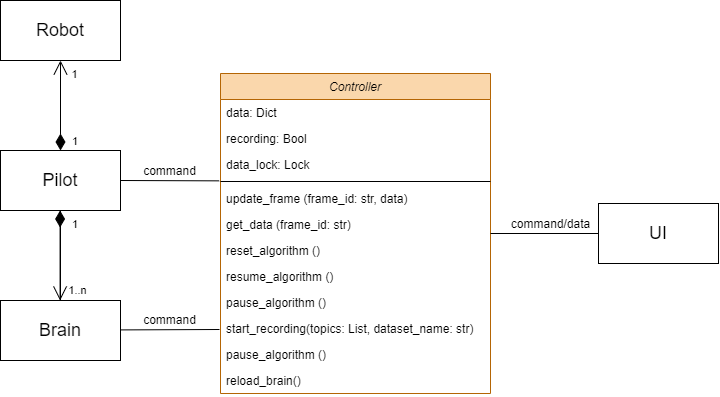
\includegraphics[width=.7\linewidth]{img/controlleruml}
  \caption{Diagrama de clases UML del componente Controlador}
  \label{fig:controluml}
\end{figure}

El controlador tiene dos modos de conexión con la capa de visualización: conexión local mediante objetos de Python y conexión remota a través de \textit{sockets} de Python. Esta conexión permite que la capa de lógica y la capa de visualización se ejecuten de forma distribuida en computadores diferentes, útil para liberar de cómputo a procesadores embebidos. En la sección \ref{sec:headless} se detalla este comportamiento.

\subsection{Grabación de \textit{datasets}}
\label{sec:redata}

El módulo de grabación de datasets, 

\subsection{Interfaz de usuario - GUI}
\label{sec:ui}

Con todos los elementos de lógica y control listos, se necesita un mecanismo para permitir al usuario final interactuar con todas las funcionalidades que ofrece la plataforma. Para éste propósito existen las interfaces de usuario o UI. Las interfaces de usuario pueden ser de diferentes tipos: gráficas (GUI), por línea de comandos (CLI), gráfica en terminal (TUI), etc. Para este proyecto se han desarrollado dos de ellas: el GUI y un TUI como prueba de concepto.

La vista principal de BehaviorStudio se puede ver en la Figura \ref{fig:mainview}. Este interfaz está dividido en dos bloques principales: la barra de herramientas (izquierda) y la visualización (derecha). A continuación se desgranan todos los componentes uno por uno.

\begin{figure}
  \centering
  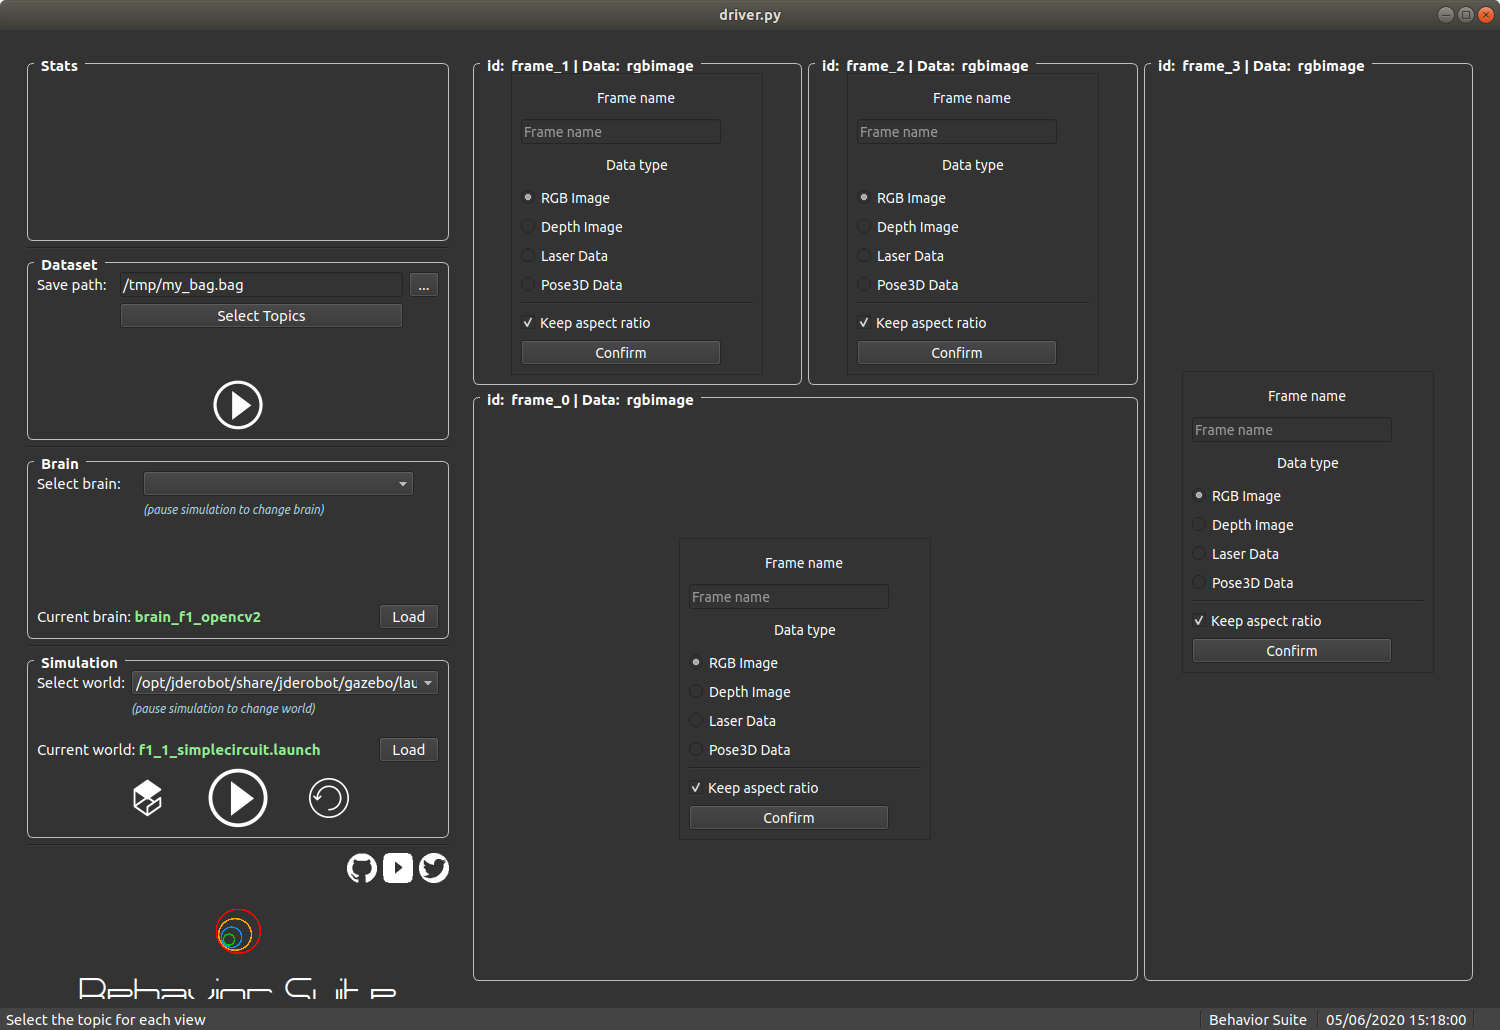
\includegraphics[width=1\linewidth]{img/main_window}
  \caption{Vista principal de BehaviorStudio}
  \label{fig:mainview}
\end{figure}

\subsubsection{Barra de herramientas}

La parte izquierda de la vista principal de BehaviorStudio contiene una barra de herramientas que permite al usuario interactuar con el sistema. Esta barra de herramientas ofrece toda la funcionalidad que el usuario podrá llevar a cabo mediante los diferentes botones que la componen. Como se puede observar en la Figura \ref{fig:toolbar}, la barra de herramientas está dividida en secciones agrupadas por funcionalidad. La primera sección titulada \textit{Stats} está diseñada para mostrar información sobre la aplicación, como consumos de memoria y CPU, estado de la conexión con el robot, tiempo de ejecución, etc.

La sección de grabación de datasets, titulada \textit{Dataset}, permite al usuario controla la grabación de conjuntos de datos a partir de \textit{topics} de ROS. Como se mencionó en secciones anteriores, la grabación de los \textit{datasets} se realiza mediante ROSBags, por lo que el usuario deberá indicar una ubicación y un nombre para el archivo de salida \texttt{.bag}, y los \textit{topics} de ROS activos que desea grabar. Una vez proporcionada esa información mediante los botones proporcionados por el GUI, el usuario podrá comenzar o detener la grabación del \textit{dataset} con el botón \textit{play} disponible.

\begin{figure}
  \centering
  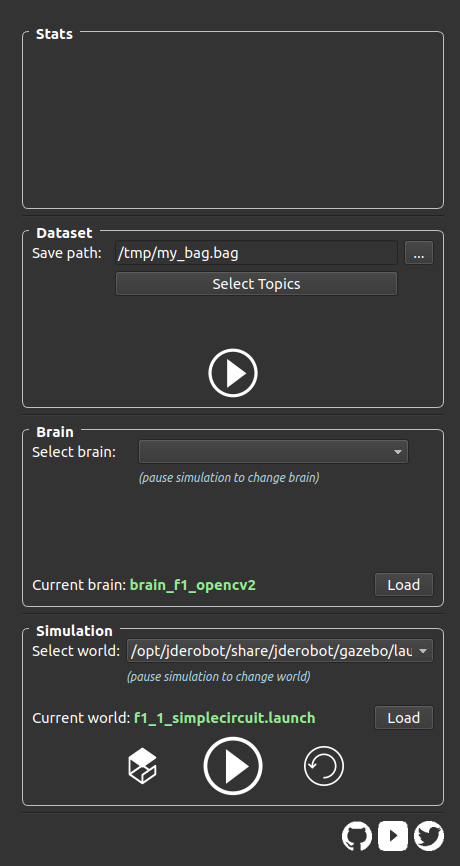
\includegraphics[width=.4\linewidth]{img/toolbar}
  \caption{Barra de herramientas de BehaviorStudio}
  \label{fig:toolbar}
\end{figure}


La sección titulada como \textit{Brain} es una de las dos más importantes de esta barra de herramientas. Con ella, el usuario podrá cargar diferentes cerebros (o controladores visuales) para el robot, en tiempo de ejecución. El desplegable ofrecerá una lista de cerebros disponibles para el robot en uso, pudiendo elegir el usuario el que desee probar en cada momento. Para poder realizar la carga en tiempo de ejecución, el algoritmo que estuviera ejecutando (si hubiera alguno) deberá estar pausado.

La sección de control del algoritmo, titulada como \textit{Simulation}, permite que el usuario pueda cargar diferentes entornos de ejecución simulados (diferentes mundos con diferentes robots), además de ofrecer tres botones para el control tanto del simulador como del algoritmo (cerebro) en ejecución:

\begin{itemize}
    \item El botón con el logo de gazebo, ejecuta o mata el cliente del simulador Gazebo en función de si este ya estaba ejecutando o no. Esto es útil para computadores con poca potencia gráfica, ya que alivia a la CPU para centrarse en la ejecución eficiente del algoritmo. Dado que el GUI de BehaviorStudio ya ofrece visualiación de los diferentes sensores, se puede prescindir del cliente del simulador.
    \item El botón con el icono de \textit{play}, permite ejecutar, pausar y resumir un algoritmo concreto especificado en la sección de la barra de herramientas \textit{Brain}. Como se ha explicado más arriba, la carga de cerebros en tiempo de ejecución sólo es posible si el algoritmo está pausado; este botón sirve para este propósito.
    \item El botón con el icono de una flecha circular sirve para reiniciar el entorno de ejecución simulado. Si el algoritmo del usuario no funciona de forma adecuada y ha provocado un estado no deseado en el entorno simulado (el coche se ha salido de la carretera, ha chocado, etc.), éste puede reiniciar la simulación devolviendo el robot a la posición original cuando se cargó el entorno simulado.
\end{itemize}

Por último, en la parte baja de la barra de herramientas hay botones para acceder a las diferentes redes sociales del proyecto.

Todas estas herramientas mencionadas se comunican con el sistema mediante el controlador explicado en la sección \ref{sec:controller}. De tal forma que cada acción que el usuario realiza en el interfaz de usuario, se traduce a un comando que llegará al sistema para llevar a cabo dicha acción.

\subsubsection{Zona de visualización}

\begin{figure}
  \centering
  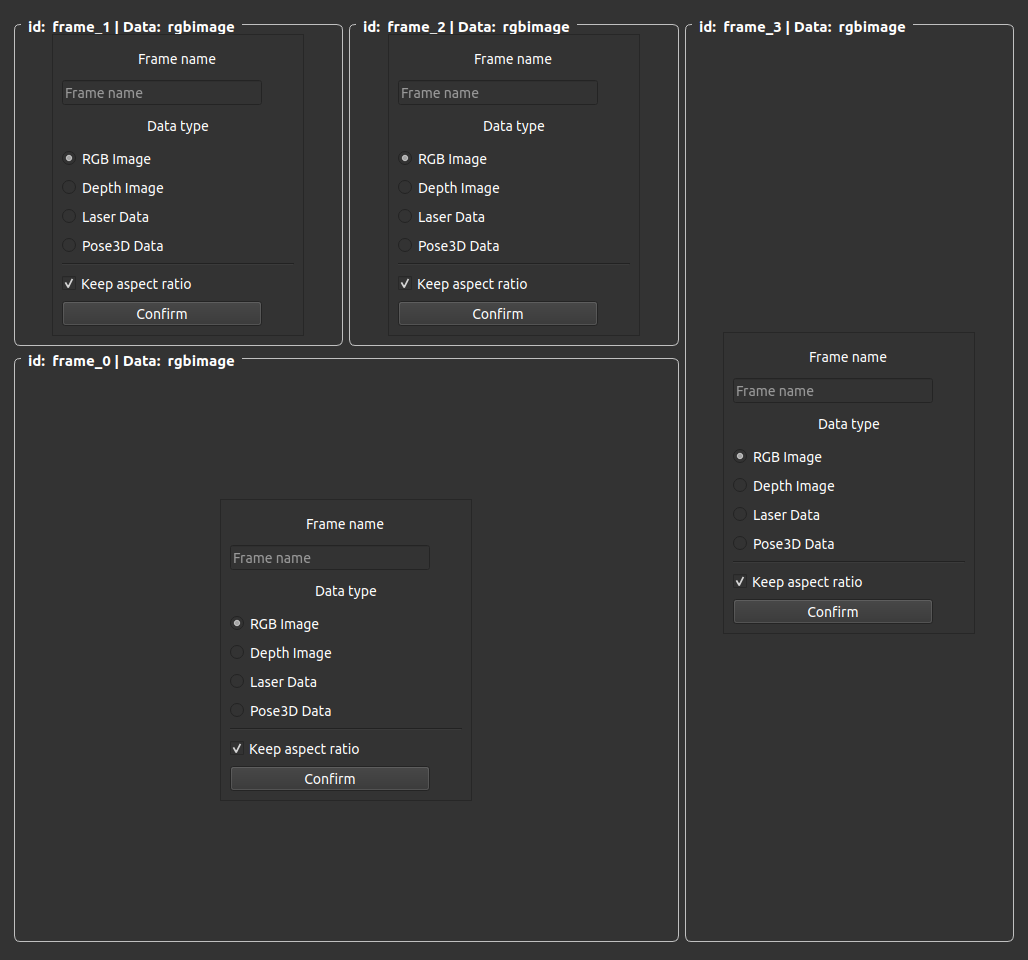
\includegraphics[width=.6\linewidth]{img/layout}
  \caption{Zona de visualización de BehaviorStudio}
  \label{fig:layout}
\end{figure}

El otro gran bloque de esta este GUI es el de visualiación. Esta parte del interfaz de usuario está diseñado para la representación de la información sensorial que ofrece el robot, como las imágenes capturadas por las cámaras RGB, la información de profundidad ofrecida por las cámaras RGBD, la información de distancia de los láseres, o la odometría del robot. 

El bloque de visualización está subdividido en cuadros o \textit{frames}, que son totalmente configurables por el usuario. La disposición de estos cuadros es una rejilla de 3x3 que puede ser dispuesta a placer. En la Figura \ref{fig:matrix_layout} se incluye un esquema para ilustrar la naturaleza configurable de estas vistas. La Figura \ref{fig:matrix_layout} (a) muestra la rejilla de 3x3 mencionada con coordenadas, la (b) muestra una configuración de ejemplo para ilustrar que una vista puede ocupar varias casillas y la (c) muestra la configuración por defecto de la plataforma. Para ilustrar la cómo se codifica la disposición de la Figura \ref{fig:matrix_layout} (b), se incluye el Fragmento \ref{yml_layout}

\begin{tabular}{c}
\begin{lstlisting}[caption={Ejemplo de configuración de la visualización},label=yml_layout] 

Frame_0:
    Name: "Camera0"
    Geometry: [0, 1, 1, 1]
    Data: rgbimage

Frame_1:
    Name: "Camera1"
    Geometry: [1, 2, 2, 2]
    Data: rgbimage
    
\end{lstlisting}
\end{tabular}

Como se puede ver, cada cuadro de visualización requiere de un nombre, una geometría y un tipo de dato por defecto. El nombre es importante ya que será el que conecte la lógica del cerebro con la visualización en el GUI. El nombre indicado en esta configuración será el mismo que el usuario tendrá que utilizar en el código del cerebro (Fragmento \ref{brainex} línea 16) cuando quiera mostrar la información sensorial en un cuadro determinado. La geometría indica la disposición de cada cuadro en la rejilla de 3x3 mencionada arriba. En el ejemplo del Fragmento \ref{yml_layout}, en la línea 3, se indica que el primer cuadro de visualización deberá estar posicionado en la coordenada (0,1) con un tamaño (o \textit{span}) de 1 posición en horizontal y 1 posición en vertical; por su parte, en la línea 8 se especifica que el segundo cuadro de visualización deberá estar posicionado en la coordenada (1,2) con un tamaño en horizontal y vertical de dos posiciones. El tipo de dato indica la información que se representará en ese cuadro: imágenes RGB, imágenes DEPTH, información de laser, etc.

\begin{figure}
	\begin{center}
		\subfloat[]{\label{fig:beast}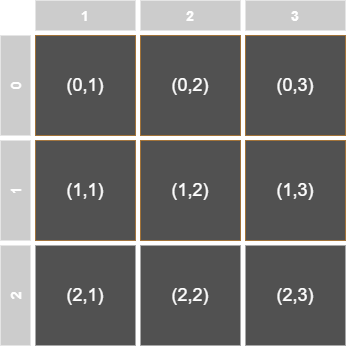
\includegraphics[width=.33\linewidth]{img/matrix_schema.png}}
		\hspace{0.1cm}
		\subfloat[]{\label{fig:stanford_cart}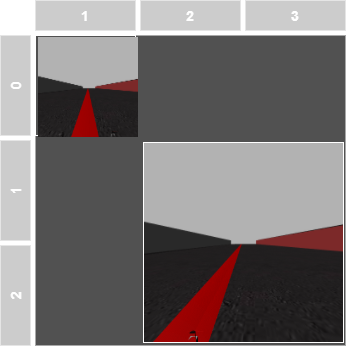
\includegraphics[width=.3\linewidth]{img/layout1.png}}
		\hspace{0.1cm}
		\subfloat[]{\label{fig:stanford_cart}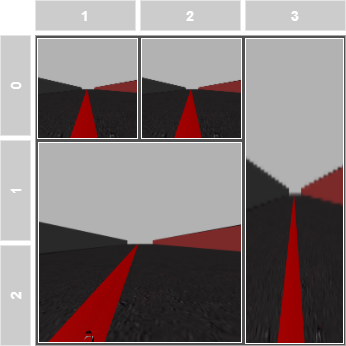
\includegraphics[width=.3\linewidth]{img/default_layout.png}}
	\end{center}	
	\centering
	\captionsetup{justification=centering,margin=0.1cm}
	\caption{(a) Rejilla de distribución de vistas. (b) Disposición de ejemplo. (c) Disposición por defecto }
	\label{fig:matrix_layout}
\end{figure}

Una vez que el usuario haya configurado las vistas a su gusto, cuando lance la aplicación verá algo similar a lo mostrado en la Figura \ref{fig:mainview}. Como se ve, en esta vista no aparece la información de ningún sensor; esto es debido a que el GUI no mostrará información sensorial hasta que no haya un algoritmo en ejecución. Cuando se ordene a la aplicación ejecutar el algoritmo de control el usuario podrá observar la información sensorial en pantalla. Cabe destacar que los diferentes cuadros de visualización pueden reconfigurarse mientras se está ejecutando un algoritmo para mostrar otros datos diferentes. Como se puede ver en la Figura \ref{fig:frame}, tanto el nombre del cuadro como el tipo de dato podrá configurarse desde el GUI, sobreescribiendo lo indicado en el fichero de configuración con el que se lanzó la aplicación. Esto es especialmente útil si, por ejemplo, se desea utilizar un cuadro de visualización más grande para mostrar más detalles de algún sensor sin necesidad de tener que reiniciar la aplicación.

\begin{figure}
  \centering
  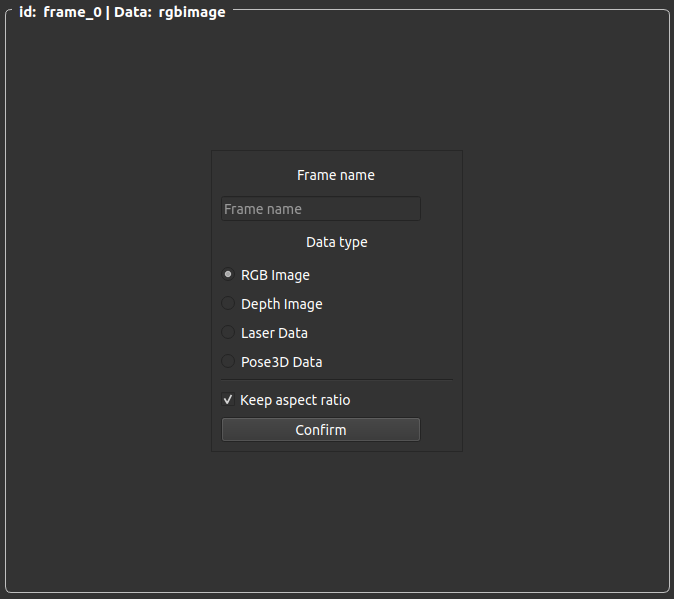
\includegraphics[width=.8\linewidth]{img/frame}
  \caption{Cuadro de visualización sensorial de BehaviorStudio}
  \label{fig:frame}
\end{figure}

\subsubsection{Interfaz por terminal - TUI}

Otro tipo de interfaz de usuario es el TUI o \textit{Terminal User Interface}. Básicamente, un TUI sirve para exactamente lo mismo que un GUI (\textit{Graphic User Interface}) pero pintado sobre una consola en lugar de con una librería gráfica basada en ventanas. El uso de TUI supone una ventaja en dos frentes: en aplicaciones minimalistas donde hay pocas (o ninguna herramienta) con las que el usuario pueda interactuar (por ejemplo los programa \textit{htop}, \textit{nvtop} o \textit{ctop} disponibles en los sistemas Linux) ahorrando tiempo de desarrollo de interfaces más complejas; o en aplicaciones embebidas que se ejecuten en sistemas pequeños con menor capacidad de cómputo que un ordenador sobremesa, para disponer de una capa de visualización con la que poder interactuar con el sistema.

En BehaviorStudio se ha desarrollado una prueba de concepto de un TUI, con el objetivo de disponer un interfaz gráfico con el que interactuar con el sistema, a bordo del robot. Dado que este tipo de interfaces no requiere de mucha potencia gráfica al ser representados en un terminal, es posible que coexista con el algoritmo de control (que se llevará la mayor parte de la potencia de cómputo). En el Anexo \ref{an:tui} se detalla un poco más el TUI desarrollado.

\section{Modo de ejecución distribuido}
\label{sec:headless}

En la sección anterior se ha descrito la interfaz de usuario desarrollada para BehaviorStudio tanto en formato GUI como en formato TUI. Dado que el sistema va a ser ejecutado en una placa de procesamiento pequeña como la Jetson Nano, es lógico pensar que sería un desperdicio de recursos el implementar una interfaz de usuario gráfica de las características de las desarrolladas para la plataforma BehaviorStudio. Como alternativa, se puede implementar un TUI para la interacción con el sistema; sin embargo, esto supone un gran inconveniente: no se pueden visualizar las imágenes de la cámara del robot. Dado que este proyecto trata de resolver el problema de la conducción autónoma mediante controladores visuales, ser capaz de depurar los algoritmos que gobiernan al robot si poder ver la información de las cámaras sería una tarea muy complicada. Es por este motivo que se decide implementar un sistema de visualización distribuido, que ha sido bautizado como modo \textit{headless}, para obtener lo mejor de ambos mundos: no derrochar recursos del procesador embebido en representar datos sensoriales, y poder visualizar los datos sensoriales en tiempo de ejecución.

La idea principal de este modo de ejecución es que la capa de lógica (el cerebro) se ejecute en el robot, mientras que la capa de visualización se ejecute en un computador más potente sin necesidad de destinar recursos computacionales a la representación de datos en pantalla. En el caso de este proyecto esto es especialmente importante, ya que la librería de gráficos utilizada (PyQt) es bastante pesada. En la Figura \ref{fig:headless} se propone la arquitectura de esta modo \textit{headless}.

\begin{figure}
  \centering
  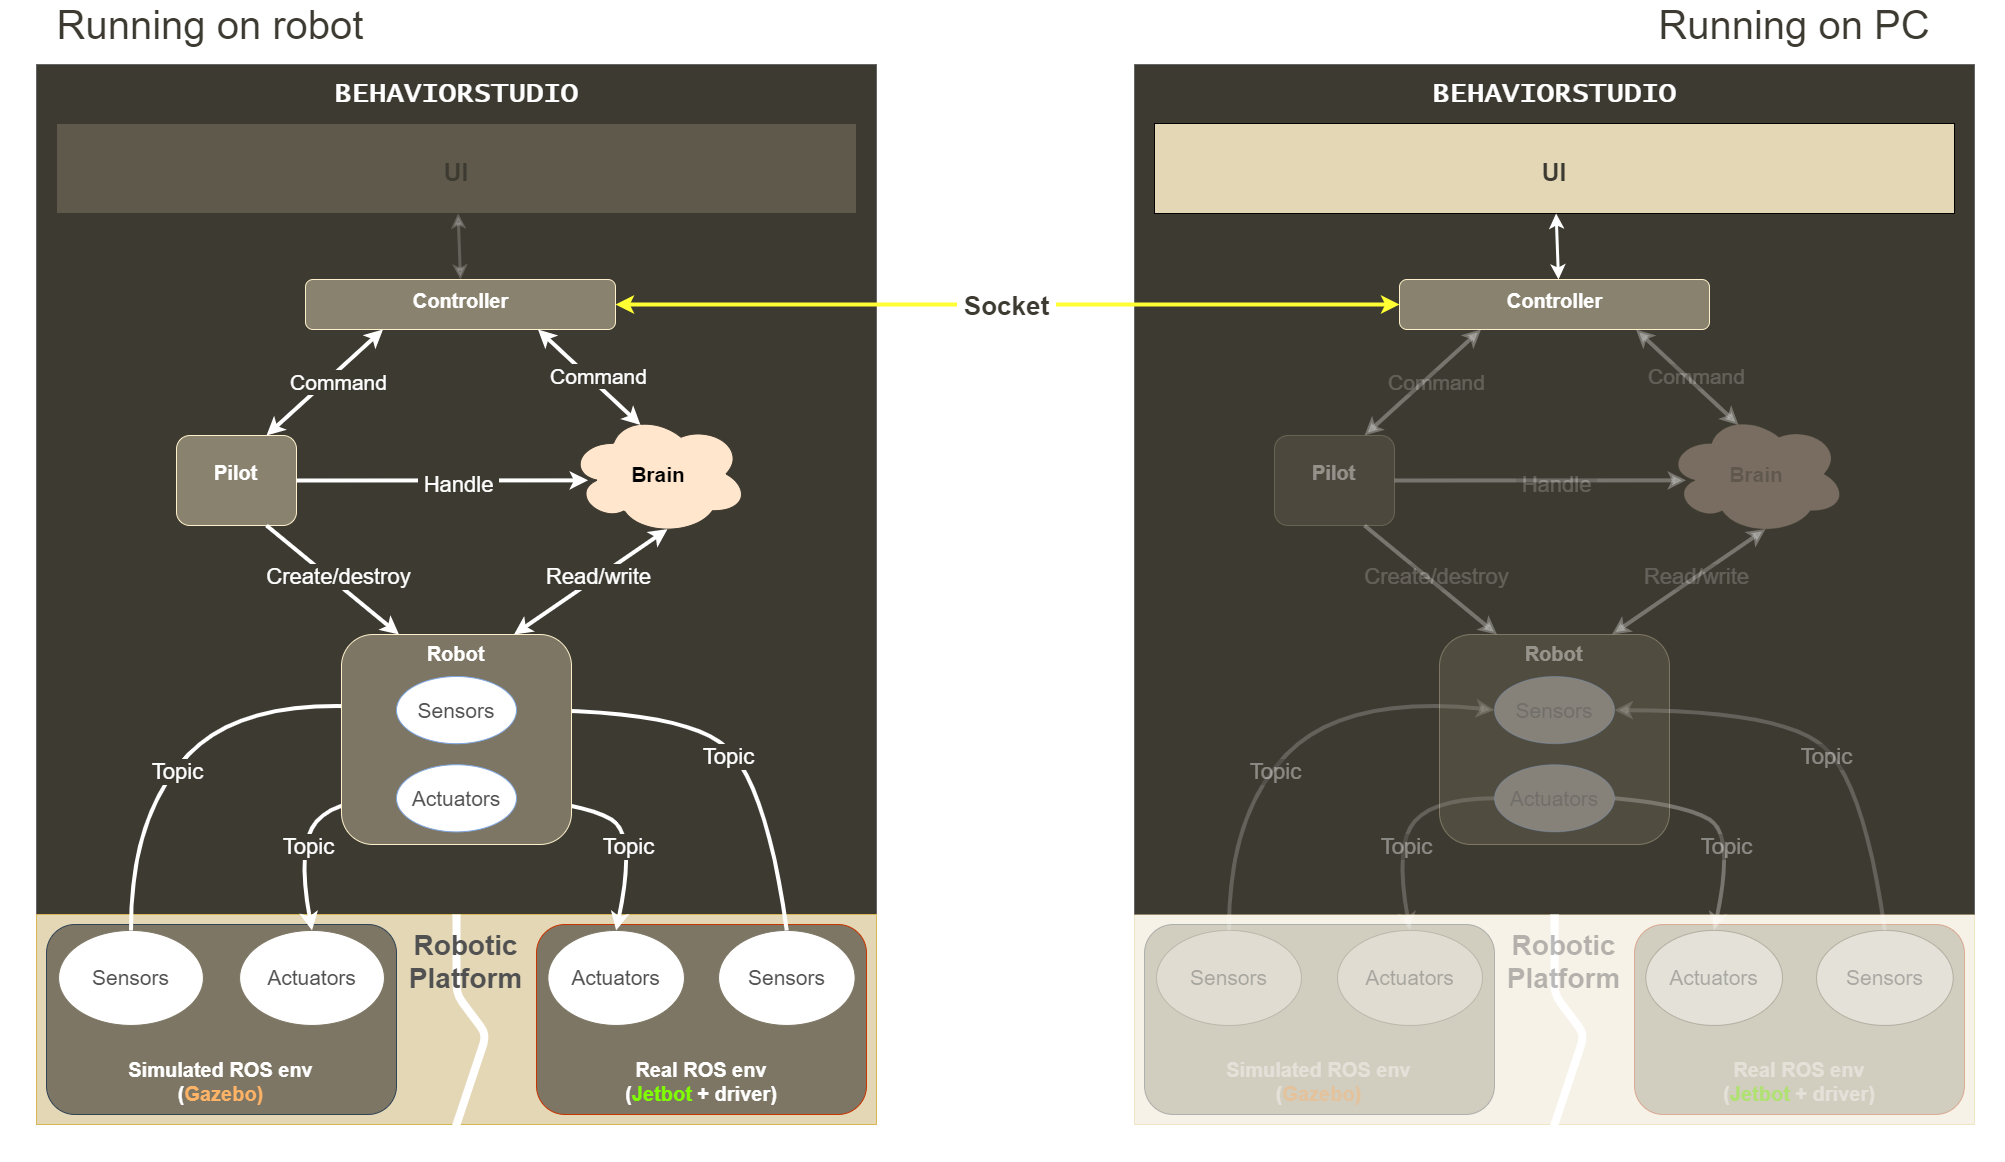
\includegraphics[width=1\linewidth]{img/headless.png}
  \caption{Arquitectura del modo \textit{headless} de BehaviorStudio}
  \label{fig:headless}
\end{figure}

Se puede observar que la arquitectura de la aplicación es la misma que la mostrada en la Figura \ref{fig:architecture}, pero duplicada. Esta representación ilustra que son dos instancias de la misma aplicación las que corren tanto en el robot como en el PC de forma distribuida, pero con partes desactivadas. La figura de la izquierda ilustra la instancia que se ejecuta en el robot, donde se puede ver que la capa de visualización está desactivada, mientras que la parte de la lógica y el controlador están activos. En el esquema de la derecha que se ejecuta en el PC, se observa el caso contrario: la capa de lógica está desactivada mientras que la capa de visualización y el controlador no. Este diseño está pensado para que haya una comunicación entre los controladores de ambas instancias de modo que el robot pueda enviar la información sensorial al PC que ejecuta la visualización, y el usuario pueda interactuar con el robot de igual manera. Para llevar a cabo esta comunicación entre instancias, se hace uso de \textit{sockets} de Python. Estos \textit{sockets} permiten que dos piezas de \textit{software} puedan intercambiar información a través de la red mediante un protocolo de comunicaciones determinado basado en TCP o UDP. De esta forma, el intercambio entre los datos sensoriales y los comandos del usuario se produce por este medio.

El protocolo de comunicación escogido en este caso es el UDP, ya que se requiere que el sistema sea reactivo. El protocolo UDP se caracteriza por tener menos latencia en el paso de mensajes y por la velocidad de envío de paquetes. Al contrario que TCP, UDP no tiene un mecanismo de seguridad para asegurar que el paquete que se ha enviado por la red ha llegado a su destino, por lo que se pueden perder paquetes sin opción de recuperación. Dado que en el problema que se está tratando se toman decisiones en cada iteración, no es tan crítico la pérdida de paquetes, ya que en pocos milisegundos llegará el siguiente con otros comandos para el robot. En la actualidad, las redes modernas son suficientemente veloces como para que el aporte de velocidad de UDP sea despreciable, no obstante la latencia es un factor crítico en estos sistemas, ya que es necesario que las decisiones tomadas por el algoritmo de control no se demoren demasiado.

\section{Validación experimental}

Como se explicó en la introducción, BehaviorStudio es una plataforma para la ejecución de comportamientos complejos en robots tanto reales como simulados. Una vez desarrollada la aplicación, se requiere de una validación de su funcionamiento más allá de los test unitarios propios de la aplicación. Para este propósito, se ha construido el llamado: piloto explícito. Este piloto es un controlador visual no neuronal basado en operaciones con imágenes mediante el uso de la librería OpenCV en un entorno simulado. Concretamente, el algoritmo realiza un filtro de color sobre la imagen que recibe del robot, donde segmenta la línea central del circuito que ha de seguir. Con la información de la imagen binaria segmentada, se calculan 2 segmentos pertenecientes a la línea segmentada (los que unen la parte baja y media de la imagen, y los que unen la parte media con el horizonte) y se calculan las pendientes de estos para determinar si el robot se encuentra frente a una recta o a una curva. Esto junto a un controlador PID para corregir la trayectoria del robot, hace que el éste sea capaz de completar el circuito de forma autónoma sin salirse de la pista. 

Además de ese piloto explícito, se ha creado otro piloto no neuronal a modo de títere que hace que el robot gire sobre sí mismo, y se ha refactorizado un cerebro neuronal de clasificación basado en el trabajo de Vanessa Fernández\footnote{\url{https://github.com/RoboticsLabURJC/2017-tfm-vanessa-fernandez}}, para ajustarlo al formato de cerebro explicado en la sección \ref{sec:brainnets}. Estos tres cerebros (el explícito, el títere y el neuronal) se utilizan para probar los cambios de cerebro en tiempo de ejecución de la plataforma. Además, dado que el entorno de simulación utilizado hace uso de robots que implementan interfaces ROS, es posible la validación del resto de funcionalidades de la aplicación como la grabación de \textit{datasets}, el cambio de circuitos en tiempo de ejecución y el cambio de vistas de los diferentes sensores. En la web de BehaviorStudio\footnote{\url{https://jderobot.github.io/BehaviorStudio/quick_start/}} se explican todas sus funcionalidades ilustrándolas con pequeñas imágenes en movimiento creadas para esta validación experimental. También está condensado en un corto vídeo en Youtube\textcolor{red}{añadir video de behaviors}

Con todos los elementos dispuestos, se realiza la validación experimental con los siguientes experimentos (el \checkmark indica que la prueba funcionó con éxito):

\begin{itemize}
    \item Carga de la aplicación con la configuración por defecto y el piloto explícito como cerebro inicial. \checkmark
    \item Ejecución del cerebro explícito para comprobar las conexiones con el robot y la plataforma a nivel de sensores y actuadores. \checkmark
    \item Validación de la visualización sensorial a través de las imágenes aportadas por el robot en la zona de visualización de la plataforma. \checkmark
    \item Pruebas de control de ejecución del cerebro: pausa y resumen. \checkmark
    \item Pruebas de control de la simulación: carga y descarga del cliente \textit{gzclient} y reinicio de la simulación. \checkmark
    \item Pruebas de grabación de \textit{datasets} incluyendo la información de la cámara y de los comandos de velocidad. \checkmark
    \item Pruebas de intercambio de cerebros entre el piloto explícito, el piloto títere y el piloto neuronal. \checkmark
    \item Pruebas de modificación de código fuente del piloto títere y recarga del cerebro ambos en tiempo de ejecución. \checkmark
\end{itemize}

Cabe destacar que la infraestructura utilizada para esta validación proviene del proyecto de \textit{software} libre JdeRobot\footnote{\url{https://jderobot.github.io}}; tanto los robots como los circuitos simulados.

Resultado de esta validación fue el correcto funcionamiento de todas las partes de la aplicación para entornos simulados. Casi todas las funcionalidades expuestas en los objetivos fueron cubiertas con éxito; no obstante, BehaviorStudio está diseñado para funcionar también con robots reales. En la siguiente sección se cubre este asunto, con la explicación del otro gran objetivo de este proyecto: conducción autónoma en un robot real mediante un controlador visual basado en \textit{deep learning}. Además, los experimentos de los algoritmos llevados a cabo en esa etapa cubren también la validación del funcionamiento de BehaviorStudio con las partes que esta prueba no cubre; a saber: funcionamiento con robots reales y funcionamiento del modo distribuido (\textit{headless}).
